% !TeX spellcheck = en_US
% !TeX encoding = UTF-8
% !TeX root = ../document.tex


\renewcommand\thechapter{A}
\chapter{Appendix}

\section{Monte Carlo Datasets}
\label{app:mc_datasets}

\subsection{Sample Name}
Most of the samples follow a consistent naming scheme. The name contains the simulated physics process, the mass range, center-of-mass energy (\SI{13}{\TeV}) and an abbreviation for the generator name.
Possible generator abbreviations are: \texttt{AM} for MadGraph\_aMC@NLO\cite{Alwall:automatedcomputationtreea}, \texttt{BM} for BlackMax\cite{Dai:BlackMaxblackhole}, \texttt{CA} for CalcHEP\cite{Belyaev:CalcHEP34collider}, \texttt{MG} for MadGraph\cite{Alwall:MadGraph5}, \texttt{P8} for Pythia 8\cite{Sjoestrand:BriefIntroductionPYTHIA}, \texttt{PH} for POWHEG BOX\cite{Frixione:MatchingNLOQCDa,Alioli:generalframeworkimplementing}, and \texttt{SP} for Sherpa\cite{Gleisberg:EventgenerationSHERPA}.

Example name "\texttt{DYJetsToLL\_M-5to50\_HT-200to400\_13TeV\_ext1\_MG}":
\begin{itemize}
\item \texttt{\underline{DYJetsToLL}\_M-5to50\_HT-200to400\_13TeV\_ext1\_MG}: Sample contains a simulation of the Drell-Yan process with two leptons in the final state
\item \texttt{DYJetsToLL\_\underline{M-5to50}\_HT-200to400\_13TeV\_ext1\_MG}: Sample is binned in the di-lepton mass (optional), this sample contains masses between \SI{5}{\GeV} and \SI{50}{\GeV}
\item \texttt{DYJetsToLL\_M-5to50\_\underline{HT-200to400}\_13TeV\_ext1\_MG}: Sample is additionally binned in the jet $H_t = p_T$ (optional), containing a range of \SI{200}{\GeV} to \SI{400}{\GeV}
\item \texttt{DYJetsToLL\_M-5to50\_HT-200to400\_\underline{13TeV}\_ext1\_MG}: The center of mass energy is $\sqrt{s} = \SI{13}{\TeV}$
\item \texttt{DYJetsToLL\_M-5to50\_HT-200to400\_13TeV\_\underline{ext1}\_MG}:
 Sample is an extension sample (optional), produced in addition to an existing sample with the same name in order to reduce statistical uncertainties
\item \texttt{DYJetsToLL\_M-5to50\_HT-200to400\_13TeV\_ext1\_\underline{MG}}:
 Sample was produced using the Madgraph generator
\end{itemize}

\pagebreak
\subsection{List}
{
    \small
    \def\arraystretch{1}
    \begin{longtable}{l l S[table-figures-decimal = 3, table-figures-exponent = 2, round-mode = figures, round-precision = 3] S[table-figures-decimal = 2, table-figures-exponent = 0, round-mode = places, round-precision = 2] l S[table-figures-decimal = 2, table-figures-exponent = 0, round-mode = places, round-precision = 2, round-minimum = 0.01, table-comparator = true] S[table-figures-integer = 9, table-figures-decimal = 0, table-figures-exponent = 0]}
\toprule
{Process} & {Dataset Name} & {Cross Section (\si{\pico\barn})} & {$k$-factor} & {Order} & {Filter Eff.} & {Events} \\
\midrule
\endhead
\multirow{35}{*}{DrellYan} & \texttt{DYJetsToLL\_M-5to50\_TuneCUETP8M1\_13TeV-madgraphMLM-pythia8} & 71310.0000000000 & 1.2300000000 & LO $\rightarrow$ NLO & 1.0000000000 & 8771481 \\
 & \texttt{DYJetsToLL\_M-5to50\_HT-100to200\_TuneCUETP8M1\_13TeV-madgraphMLM-pythia8} & 224.2000000000 & 1.2300000000 & LO $\rightarrow$ NLO & 1.0000000000 & 1018459 \\
 & \texttt{DYJetsToLL\_M-5to50\_HT-100to200\_TuneCUETP8M1\_13TeV-madgraphMLM-pythia8 (ext1)} & 224.2000000000 & 1.2300000000 & LO $\rightarrow$ NLO & 1.0000000000 & 8145474 \\
 & \texttt{DYJetsToLL\_M-5to50\_HT-200to400\_TuneCUETP8M1\_13TeV-madgraphMLM-pythia8} & 37.1900000000 & 1.2300000000 & LO $\rightarrow$ NLO & 1.0000000000 & 1025157 \\
 & \texttt{DYJetsToLL\_M-5to50\_HT-200to400\_TuneCUETP8M1\_13TeV-madgraphMLM-pythia8 (ext1)} & 37.1900000000 & 1.2300000000 & LO $\rightarrow$ NLO & 1.0000000000 & 2020586 \\
 & \texttt{DYJetsToLL\_M-5to50\_HT-400to600\_TuneCUETP8M1\_13TeV-madgraphMLM-pythia8} & 3.5810000000 & 1.2300000000 & LO $\rightarrow$ NLO & 1.0000000000 & 1012963 \\
 & \texttt{DYJetsToLL\_M-5to50\_HT-600toInf\_TuneCUETP8M1\_13TeV-madgraphMLM-pythia8} & 1.1240000000 & 1.2300000000 & LO $\rightarrow$ NLO & 1.0000000000 & 1019394 \\
 & \texttt{DYJetsToLL\_M-5to50\_HT-600toInf\_TuneCUETP8M1\_13TeV-madgraphMLM-pythia8 (ext1)} & 1.1240000000 & 1.2300000000 & LO $\rightarrow$ NLO & 1.0000000000 & 1924359 \\
 & \texttt{DYJetsToLL\_M-50\_TuneCUETP8M1\_13TeV-madgraphMLM-pythia8} & 4895.0000000000 & 1.2300000000 & LO $\rightarrow$ NNLO & 1.0000000000 & 8877130 \\
 & \texttt{DYJetsToLL\_M-50\_TuneCUETP8M1\_13TeV-madgraphMLM-pythia8 (ext1)} & 4895.0000000000 & 1.1800000000 & LO $\rightarrow$ NNLO & 1.0000000000 & 240499997 \\
 & \texttt{DYJetsToLL\_M-50\_HT-100to200\_TuneCUETP8M1\_13TeV-madgraphMLM-pythia8} & 147.4000000000 & 1.2300000000 & LO $\rightarrow$ NLO & 1.0000000000 & 2564547 \\
 & \texttt{DYJetsToLL\_M-50\_HT-100to200\_TuneCUETP8M1\_13TeV-madgraphMLM-pythia8 (ext1)} & 147.4000000000 & 1.2300000000 & LO $\rightarrow$ NLO & 1.0000000000 & 7829684 \\
 & \texttt{DYJetsToLL\_M-50\_HT-200to400\_TuneCUETP8M1\_13TeV-madgraphMLM-pythia8} & 42.7500000000 & 1.4400000000 & LO $\rightarrow$ NLO & 1.0000000000 & 962195 \\
 & \texttt{DYJetsToLL\_M-50\_HT-400to600\_TuneCUETP8M1\_13TeV-madgraphMLM-pythia8} & 5.6780000000 & 1.2300000000 & LO $\rightarrow$ NLO & 1.0000000000 & 1069003 \\
 & \texttt{DYJetsToLL\_M-50\_HT-400to600\_TuneCUETP8M1\_13TeV-madgraphMLM-pythia8 (ext1)} & 5.6780000000 & 1.2300000000 & LO $\rightarrow$ NLO & 1.0000000000 & 3431833 \\
 & \texttt{DYJetsToLL\_M-50\_HT-600toInf\_TuneCUETP8M1\_13TeV-madgraphMLM-pythia8} & 2.2100000000 & 1.1400000000 & LO $\rightarrow$ NLO & 1.0000000000 & 1031103 \\
 & \texttt{DYJetsToLL\_M-50\_HT-600toInf\_TuneCUETP8M1\_13TeV-madgraphMLM-pythia8 (ext1)} & 2.2100000000 & 1.1400000000 & LO $\rightarrow$ NLO & 1.0000000000 & 4058472 \\
 & \texttt{ZToEE\_NNPDF30\_13TeV-powheg\_M\_120\_200} & 19.3200000000 & {-} & NLO & 1.0000000000 & 100000 \\
 & \texttt{ZToEE\_NNPDF30\_13TeV-powheg\_M\_200\_400} & 2.7310000000 & {-} & NLO & 1.0000000000 & 100000 \\
 & \texttt{ZToEE\_NNPDF30\_13TeV-powheg\_M\_400\_800} & 0.2410000000 & {-} & NLO & 1.0000000000 & 100000 \\
 & \texttt{ZToEE\_NNPDF30\_13TeV-powheg\_M\_800\_1400} & 0.0167800000 & {-} & NLO & 1.0000000000 & 100000 \\
 & \texttt{ZToEE\_NNPDF30\_13TeV-powheg\_M\_1400\_2300} & 0.0013900000 & {-} & NLO & 1.0000000000 & 100000 \\
 & \texttt{ZToEE\_NNPDF30\_13TeV-powheg\_M\_2300\_3500} & 0.0000894800 & {-} & NLO & 1.0000000000 & 100000 \\
 & \texttt{ZToEE\_NNPDF30\_13TeV-powheg\_M\_3500\_4500} & 0.0000041350 & {-} & NLO & 1.0000000000 & 100000 \\
 & \texttt{ZToEE\_NNPDF30\_13TeV-powheg\_M\_4500\_6000} & 0.0000004560 & {-} & NLO & 1.0000000000 & 99000 \\
 & \texttt{ZToEE\_NNPDF30\_13TeV-powheg\_M\_6000\_Inf} & 0.0000000207 & {-} & NLO & 1.0000000000 & 97600 \\
 & \texttt{ZToMuMu\_NNPDF30\_13TeV-powheg\_M\_120\_200} & 19.3200000000 & {-} & NLO & 1.0000000000 & 100000 \\
 & \texttt{ZToMuMu\_NNPDF30\_13TeV-powheg\_M\_200\_400} & 2.7310000000 & {-} & NLO & 1.0000000000 & 100000 \\
 & \texttt{ZToMuMu\_NNPDF30\_13TeV-powheg\_M\_400\_800} & 0.2410000000 & {-} & NLO & 1.0000000000 & 99600 \\
 & \texttt{ZToMuMu\_NNPDF30\_13TeV-powheg\_M\_800\_1400} & 0.0170000000 & {-} & NLO & 1.0000000000 & 97600 \\
 & \texttt{ZToMuMu\_NNPDF30\_13TeV-powheg\_M\_1400\_2300} & 0.0013900000 & {-} & NLO & 1.0000000000 & 99200 \\
 & \texttt{ZToMuMu\_NNPDF30\_13TeV-powheg\_M\_2300\_3500} & 0.0000894800 & {-} & NLO & 1.0000000000 & 100000 \\
 & \texttt{ZToMuMu\_NNPDF30\_13TeV-powheg\_M\_3500\_4500} & 0.0000041350 & {-} & NLO & 1.0000000000 & 100000 \\
 & \texttt{ZToMuMu\_NNPDF30\_13TeV-powheg\_M\_4500\_6000} & 0.0000004560 & {-} & NLO & 1.0000000000 & 100000 \\
 & \texttt{ZToMuMu\_NNPDF30\_13TeV-powheg\_M\_6000\_Inf} & 0.0000000207 & {-} & NLO & 1.0000000000 & 99200 \\
\midrule
\multirow{5}{*}{Gamma} & \texttt{GJets\_HT-40To100\_TuneCUETP8M1\_13TeV-madgraphMLM-pythia8} & 20790.0000000000 & {-} & LO & 1.0000000000 & 4424830 \\
 & \texttt{GJets\_HT-100To200\_TuneCUETP8M1\_13TeV-madgraphMLM-pythia8} & 9238.0000000000 & {-} & LO & 1.0000000000 & 4877095 \\
 & \texttt{GJets\_HT-200To400\_TuneCUETP8M1\_13TeV-madgraphMLM-pythia8} & 2305.0000000000 & {-} & LO & 1.0000000000 & 10467654 \\
 & \texttt{GJets\_HT-400To600\_TuneCUETP8M1\_13TeV-madgraphMLM-pythia8} & 274.4000000000 & {-} & LO & 1.0000000000 & 2406285 \\
 & \texttt{GJets\_HT-600ToInf\_TuneCUETP8M1\_13TeV-madgraphMLM-pythia8} & 93.4600000000 & {-} & LO & 1.0000000000 & 2456253 \\
\midrule
\multirow{14}{*}{QCD} & \texttt{QCD\_Pt-50to80\_EMEnriched\_TuneCUETP8M1\_13TeV\_pythia8} & 19800000.0000000000 & {-} & LO & 0.1460000000 & 22463814 \\
 & \texttt{QCD\_Pt-50to80\_MuEnrichedPt5\_TuneCUETP8M1\_13TeV\_pythia8} & 19222500.0000000000 & {-} & LO & 0.0227600000 & 20378392 \\
 & \texttt{QCD\_Pt-80to120\_EMEnriched\_TuneCUETP8M1\_13TeV\_pythia8} & 2800000.0000000000 & {-} & LO & 0.1250000000 & 36029628 \\
 & \texttt{QCD\_Pt-80to120\_MuEnrichedPt5\_TuneCUETP8M1\_13TeV\_pythia8} & 2758420.0000000000 & {-} & LO & 0.0384400000 & 13749024 \\
 & \texttt{QCD\_Pt-120to170\_EMEnriched\_TuneCUETP8M1\_13TeV\_pythia8} & 477000.0000000000 & {-} & LO & 0.1320000000 & 36202409 \\
 & \texttt{QCD\_Pt-120to170\_MuEnrichedPt5\_TuneCUETP8M1\_13TeV\_pythia8} & 469797.0000000000 & {-} & LO & 0.0536200000 & 7971018 \\
 & \texttt{QCD\_Pt-170to300\_EMEnriched\_TuneCUETP8M1\_13TeV\_pythia8} & 114000.0000000000 & {-} & LO & 0.1650000000 & 11518871 \\
 & \texttt{QCD\_Pt-170to300\_MuEnrichedPt5\_TuneCUETP8M1\_13TeV\_pythia8} & 117989.0000000000 & {-} & LO & 0.0733500000 & 7910182 \\
 & \texttt{QCD\_Pt-300to470\_MuEnrichedPt5\_TuneCUETP8M1\_13TeV\_pythia8} & 7820.2500000000 & {-} & LO & 0.1019600000 & 7845620 \\
 & \texttt{QCD\_Pt-300toInf\_EMEnriched\_TuneCUETP8M1\_13TeV\_pythia8} & 9000.0000000000 & {-} & LO & 0.1500000000 & 7212550 \\
 & \texttt{QCD\_Pt-470to600\_MuEnrichedPt5\_TuneCUETP8M1\_13TeV\_pythia8} & 645.5280000000 & {-} & LO & 0.1224200000 & 3841262 \\
 & \texttt{QCD\_Pt-600to800\_MuEnrichedPt5\_TuneCUETP8M1\_13TeV\_pythia8} & 187.1090000000 & {-} & LO & 0.1341200000 & 3984898 \\
 & \texttt{QCD\_Pt-800to1000\_MuEnrichedPt5\_TuneCUETP8M1\_13TeV\_pythia8} & 32.3486000000 & {-} & LO & 0.1455200000 & 3666110 \\
 & \texttt{QCD\_Pt-1000toInf\_MuEnrichedPt5\_TuneCUETP8M1\_13TeV\_pythia8} & 10.4305000000 & {-} & LO & 0.1554400000 & 3938782 \\
\midrule
\multirow{2}{*}{TG} & \texttt{TGJets\_TuneCUETP8M1\_13TeV\_amcatnlo\_madspin\_pythia8} & 2.9670000000 & {-} & NLO & 1.0000000000 & 280100 \\
 & \texttt{TGJets\_TuneCUETP8M1\_13TeV\_amcatnlo\_madspin\_pythia8 (ext1)} & 2.9670000000 & {-} & NLO & 1.0000000000 & 1556996 \\
\midrule
\multirow{6}{*}{TTBar} & \texttt{TT\_TuneCUETP8M1\_13TeV-powheg-pythia8 (ext3)} & 730.0000000000 & 1.1394000000 & NLO $\rightarrow$ NNLO & 1.0000000000 & 97994442 \\
 & \texttt{TT\_TuneCUETP8M1\_13TeV-powheg-pythia8 (ext4)} & 730.0000000000 & 1.1394000000 & NLO $\rightarrow$ NNLO & 1.0000000000 & 187626200 \\
 & \texttt{TT\_Mtt-700to1000\_TuneCUETP8M1\_13TeV-powheg-pythia8} & 730.0000000000 & 1.1394000000 & NLO $\rightarrow$ NNLO & 0.0921000000 & 37285071 \\
 & \texttt{TT\_Mtt-700to1000\_TuneCUETP8M1\_13TeV-powheg-pythia8 (ext1)} & 730.0000000000 & 1.1394000000 & NLO $\rightarrow$ NNLO & 0.0921000000 & 3086786 \\
 & \texttt{TT\_Mtt-1000toInf\_TuneCUETP8M1\_13TeV-powheg-pythia8 (ext1)} & 730.0000000000 & 1.1394000000 & NLO $\rightarrow$ NNLO & 0.0247400000 & 1782160 \\
 & \texttt{TT\_Mtt-1000toInf\_TuneCUETP8M1\_13TeV-powheg-pythia8 (ext2)} & 730.0000000000 & 1.1394000000 & NLO $\rightarrow$ NNLO & 0.0247400000 & 25182267 \\
\midrule
\multirow{1}{*}{TTG} & \texttt{TTGJets\_TuneCUETP8M1\_13TeV-amcatnloFXFX-madspin-pythia8} & 3.6970000000 & {-} & NLO & 1.0000000000 & 4874116 \\
\midrule
\multirow{1}{*}{TTGG} & \texttt{TTGG\_0Jets\_TuneCUETP8M1\_13TeV\_amcatnlo\_madspin\_pythia8} & 0.0173000000 & {-} & NLO & 1.0000000000 & 1466516 \\
\midrule
\multirow{1}{*}{TTW} & \texttt{ttWJets\_13TeV\_madgraphMLM} & 0.2430000000 & {-} & LO & 1.0000000000 & 12889768 \\
\midrule
\multirow{1}{*}{TTZ} & \texttt{ttZJets\_13TeV\_madgraphMLM} & 0.2590000000 & {-} & LO & 1.0000000000 & 22157947 \\
\midrule
\multirow{2}{*}{TZQ} & \texttt{tZq\_ll\_4f\_13TeV-amcatnlo-pythia8\_TuneCUETP8M1} & 0.0758000000 & {-} & NLO & 1.0000000000 & 2996000 \\
 & \texttt{tZq\_nunu\_4f\_13TeV-amcatnlo-pythia8\_TuneCUETP8M1} & 0.1379000000 & {-} & NLO & 1.0000000000 & 984600 \\
\midrule
\multirow{3}{*}{Top} & \texttt{ST\_s-channel\_4f\_leptonDecays\_13TeV-amcatnlo-pythia8\_TuneCUETP8M1} & 3.3600000000 & {-} & NLO & 1.0000000000 & 998400 \\
 & \texttt{ST\_t-channel\_antitop\_4f\_leptonDecays\_13TeV-powheg-pythia8\_TuneCUETP8M1} & 25.3000000000 & {-} & NLO & 1.0000000000 & 1630900 \\
 & \texttt{ST\_t-channel\_top\_4f\_leptonDecays\_13TeV-powheg-pythia8\_TuneCUETP8M1} & 41.9000000000 & {-} & NLO & 1.0000000000 & 3299200 \\
\midrule
\multirow{30}{*}{W} & \texttt{WJetsToLNu\_TuneCUETP8M1\_13TeV-madgraphMLM-pythia8} & 50690.0000000000 & 1.2138000000 & LO $\rightarrow$ NNLO & 1.0000000000 & 47161328 \\
 & \texttt{WJetsToLNu\_HT-100To200\_TuneCUETP8M1\_13TeV-madgraphMLM-pythia8} & 1345.0000000000 & 1.2100000000 & LO $\rightarrow$ NLO\_W & 1.0000000000 & 10205377 \\
 & \texttt{WJetsToLNu\_HT-100To200\_TuneCUETP8M1\_13TeV-madgraphMLM-pythia8 (ext1)} & 1345.0000000000 & 1.2100000000 & LO $\rightarrow$ NLO\_W & 1.0000000000 & 28484673 \\
 & \texttt{WJetsToLNu\_HT-200To400\_TuneCUETP8M1\_13TeV-madgraphMLM-pythia8} & 359.7000000000 & 1.2100000000 & LO $\rightarrow$ NLO\_W & 1.0000000000 & 4692696 \\
 & \texttt{WJetsToLNu\_HT-200To400\_TuneCUETP8M1\_13TeV-madgraphMLM-pythia8 (ext1)} & 359.7000000000 & 1.2100000000 & LO $\rightarrow$ NLO\_W & 1.0000000000 & 14881357 \\
 & \texttt{WJetsToLNu\_HT-400To600\_TuneCUETP8M1\_13TeV-madgraphMLM-pythia8} & 48.9100000000 & 1.2100000000 & LO $\rightarrow$ NLO\_W & 1.0000000000 & 1943664 \\
 & \texttt{WJetsToLNu\_HT-600To800\_TuneCUETP8M1\_13TeV-madgraphMLM-pythia8} & 12.0500000000 & 1.2138000000 & LO $\rightarrow$ NLO\_W & 1.0000000000 & 3767766 \\
 & \texttt{WJetsToLNu\_HT-800To1200\_TuneCUETP8M1\_13TeV-madgraphMLM-pythia8} & 5.5010000000 & 1.2138000000 & LO $\rightarrow$ NLO\_W & 1.0000000000 & 1568277 \\
 & \texttt{WJetsToLNu\_HT-1200To2500\_TuneCUETP8M1\_13TeV-madgraphMLM-pythia8} & 1.3290000000 & 1.2138000000 & LO $\rightarrow$ NLO\_W & 1.0000000000 & 246239 \\
 & \texttt{WJetsToLNu\_HT-1200To2500\_TuneCUETP8M1\_13TeV-madgraphMLM-pythia8 (ext1)} & 1.3290000000 & 1.2138000000 & LO $\rightarrow$ NLO\_W & 1.0000000000 & 6709861 \\
 & \texttt{WJetsToLNu\_HT-2500ToInf\_TuneCUETP8M1\_13TeV-madgraphMLM-pythia8} & 0.0321600000 & 1.2138000000 & LO $\rightarrow$ NLO\_W & 1.0000000000 & 251982 \\
 & \texttt{WJetsToLNu\_HT-2500ToInf\_TuneCUETP8M1\_13TeV-madgraphMLM-pythia8 (ext1)} & 0.0321600000 & 1.2100000000 & LO $\rightarrow$ NLO\_W & 1.0000000000 & 2300696 \\
 & \texttt{WJetsToQQ\_HT180\_13TeV-madgraphMLM-pythia8} & 2788.0000000000 & {-} & LO & 1.0000000000 & 22689606 \\
 & \texttt{WJetsToQQ\_HT-600ToInf\_TuneCUETP8M1\_13TeV-madgraphMLM-pythia8} & 95.1400000000 & {-} & LO & 1.0000000000 & 1025100 \\
 & \texttt{WToENu\_M-200\_TuneCUETP8M1\_13TeV-pythia8} & 6.2360000000 & 1.3367300000 & LO $\rightarrow$ NNLO & 1.0000000000 & 998887 \\
 & \texttt{WToENu\_M-500\_TuneCUETP8M1\_13TeV-pythia8} & 0.2138000000 & 1.3314600000 & LO $\rightarrow$ NNLO & 1.0000000000 & 993370 \\
 & \texttt{WToENu\_M-1000\_TuneCUETP8M1\_13TeV-pythia8} & 0.0128100000 & 1.3268400000 & LO $\rightarrow$ NNLO & 1.0000000000 & 998728 \\
 & \texttt{WToENu\_M-2000\_TuneCUETP8M1\_13TeV-pythia8} & 0.0005560000 & 1.2571700000 & LO $\rightarrow$ NNLO & 1.0000000000 & 998096 \\
 & \texttt{WToENu\_M-3000\_TuneCUETP8M1\_13TeV-pythia8} & 0.0000290400 & 1.1359000000 & LO $\rightarrow$ NNLO & 1.0000000000 & 995350 \\
 & \texttt{WToENu\_M-4000\_TuneCUETP8M1\_13TeV-pythia8} & 0.0000030300 & 0.4500000000 & LO $\rightarrow$ NNLO & 1.0000000000 & 993166 \\
 & \texttt{WToMuNu\_M-200\_TuneCUETP8M1\_13TeV-pythia8} & 6.2360000000 & 1.2885300000 & LO $\rightarrow$ NNLO & 1.0000000000 & 993140 \\
 & \texttt{WToMuNu\_M-500\_TuneCUETP8M1\_13TeV-pythia8} & 0.2138000000 & 1.2725300000 & LO $\rightarrow$ NNLO & 1.0000000000 & 997511 \\
 & \texttt{WToMuNu\_M-1000\_TuneCUETP8M1\_13TeV-pythia8} & 0.0128100000 & 1.2603800000 & LO $\rightarrow$ NNLO & 1.0000000000 & 992260 \\
 & \texttt{WToMuNu\_M-2000\_TuneCUETP8M1\_13TeV-pythia8} & 0.0005560000 & 1.1725600000 & LO $\rightarrow$ NNLO & 1.0000000000 & 994764 \\
 & \texttt{WToMuNu\_M-3000\_TuneCUETP8M1\_13TeV-pythia8} & 0.0000290400 & 1.0383400000 & LO $\rightarrow$ NNLO & 1.0000000000 & 996545 \\
 & \texttt{WToMuNu\_M-4000\_TuneCUETP8M1\_13TeV-pythia8} & 0.0000030300 & 0.4086070000 & LO $\rightarrow$ NNLO & 1.0000000000 & 992708 \\
 & \texttt{WToTauNu\_M-200\_TuneCUETP8M1\_13TeV-pythia8} & 6.2360000000 & 1.3451000000 & LO $\rightarrow$ NNLO & 1.0000000000 & 991772 \\
 & \texttt{WToTauNu\_M-500\_TuneCUETP8M1\_13TeV-pythia8-tauola} & 0.2240000000 & {-} & LO & 1.0000000000 & 977384 \\
 & \texttt{WToTauNu\_M-1000\_TuneCUETP8M1\_13TeV-pythia8} & 0.0128100000 & 1.3263100000 & LO $\rightarrow$ NNLO & 1.0000000000 & 999316 \\
 & \texttt{WToTauNu\_M-2000\_TuneCUETP8M1\_13TeV-pythia8-tauola} & 0.0005560000 & {-} & LO & 1.0000000000 & 977400 \\
\midrule
\multirow{2}{*}{WG} & \texttt{WGToLNuG\_TuneCUETP8M1\_13TeV-madgraphMLM-pythia8} & 405.2710000000 & 1.2066000000 & LO $\rightarrow$ NLO & 1.0000000000 & 6102260 \\
 & \texttt{WGToLNuG\_PtG-500\_TuneCUETP8M1\_13TeV-madgraphMLM-pythia8} & 0.0117887000 & {-} & LO & 1.0000000000 & 1390140 \\
\midrule
\multirow{9}{*}{WW} & \texttt{WWTo2L2Nu\_13TeV-powheg} & 10.4800000000 & 1.1620000000 & NLO $\rightarrow$ NNLO & 1.0000000000 & 1979988 \\
 & \texttt{WWTo2L2Nu\_Mll\_200To600\_13TeV-powheg} & 10.4814000000 & 1.1620000000 & NLO $\rightarrow$ NNLO & 0.1137730000 & 200000 \\
 & \texttt{WWTo2L2Nu\_Mll\_600To1200\_13TeV-powheg} & 10.4814000000 & 1.1620000000 & NLO $\rightarrow$ NNLO & 0.0046514000 & 200000 \\
 & \texttt{WWTo2L2Nu\_Mll\_1200To2500\_13TeV-powheg} & 10.4814000000 & 1.1620000000 & NLO $\rightarrow$ NNLO & 0.0002920300 & 198400 \\
 & \texttt{WWTo2L2Nu\_Mll\_2500ToInf\_13TeV-powheg} & 10.4814000000 & 1.1620000000 & NLO $\rightarrow$ NNLO & 0.0000044310 & 38969 \\
 & \texttt{WWTo4Q\_13TeV-powheg} & 45.2000000000 & 1.1443000000 & NLO $\rightarrow$ NNLO & 1.0000000000 & 2000000 \\
 & \texttt{WWToLNuQQ\_13TeV-powheg} & 43.5300000000 & 1.1486000000 & NLO $\rightarrow$ NNLO & 1.0000000000 & 1924400 \\
 & \texttt{WWToLNuQQ\_13TeV-powheg (ext1)} & 43.5300000000 & 1.1486000000 & NLO $\rightarrow$ NNLO & 1.0000000000 & 6996000 \\
 & \texttt{WW\_DoubleScattering\_13TeV-pythia8} & 1.6400000000 & {-} & LO & 1.0000000000 & 844954 \\
\midrule
\multirow{1}{*}{WWG} & \texttt{WWG\_TuneCUETP8M1\_13TeV-amcatnlo-pythia8 (ext1)} & 0.2147000000 & {-} & NLO & 1.0000000000 & 995400 \\
\midrule
\multirow{1}{*}{WWW} & \texttt{WWW\_4F\_TuneCUETP8M1\_13TeV-amcatnlo-pythia8} & 0.2086000000 & {-} & NLO & 1.0000000000 & 240000 \\
\midrule
\multirow{1}{*}{WWZ} & \texttt{WWZ\_TuneCUETP8M1\_13TeV-amcatnlo-pythia8} & 0.1651000000 & {-} & NLO & 1.0000000000 & 248400 \\
\midrule
\multirow{4}{*}{WZ} & \texttt{WZTo1L1Nu2Q\_13TeV\_amcatnloFXFX\_madspin\_pythia8} & 10.7100000000 & {-} & NLO & 1.0000000000 & 19742520 \\
 & \texttt{WZTo1L3Nu\_13TeV\_amcatnloFXFX\_madspin\_pythia8} & 3.0330000000 & {-} & NLO & 1.0000000000 & 1703772 \\
 & \texttt{WZTo2L2Q\_13TeV\_amcatnloFXFX\_madspin\_pythia8} & 5.5950000000 & {-} & NLO & 1.0000000000 & 25704656 \\
 & \texttt{WZTo3LNu\_TuneCUETP8M1\_13TeV-powheg-pythia8} & 4.4296500000 & {-} & NLO & 1.0000000000 & 2000000 \\
\midrule
\multirow{1}{*}{WZG} & \texttt{WZG\_TuneCUETP8M1\_13TeV-amcatnlo-pythia8} & 0.0412300000 & {-} & NLO & 1.0000000000 & 997400 \\
\midrule
\multirow{1}{*}{WZZ} & \texttt{WZZ\_TuneCUETP8M1\_13TeV-amcatnlo-pythia8} & 0.0556500000 & {-} & NLO & 1.0000000000 & 249800 \\
\midrule
\multirow{5}{*}{ZToInvisible} & \texttt{ZJetsToNuNu\_HT-100To200\_13TeV-madgraph} & 280.4700000000 & 1.6300000000 & LO $\rightarrow$ NLO & 1.0000000000 & 5240199 \\
 & \texttt{ZJetsToNuNu\_HT-200To400\_13TeV-madgraph} & 78.3600000000 & 1.6200000000 & LO $\rightarrow$ NLO & 1.0000000000 & 2170249 \\
 & \texttt{ZJetsToNuNu\_HT-200To400\_13TeV-madgraph (ext1)} & 78.3600000000 & 1.6200000000 & LO $\rightarrow$ NLO & 1.0000000000 & 19007186 \\
 & \texttt{ZJetsToNuNu\_HT-400To600\_13TeV-madgraph} & 10.9440000000 & 1.4600000000 & LO $\rightarrow$ NLO & 1.0000000000 & 954435 \\
 & \texttt{ZJetsToNuNu\_HT-600ToInf\_13TeV-madgraph} & 4.2030000000 & 1.3900000000 & LO $\rightarrow$ NLO & 1.0000000000 & 1033818 \\
\midrule
\multirow{5}{*}{ZZ} & \texttt{ZZTo2L2Nu\_13TeV\_powheg\_pythia8} & 0.5644000000 & {-} & NLO & 1.0000000000 & 8785050 \\
 & \texttt{ZZTo2L2Q\_13TeV\_amcatnloFXFX\_madspin\_pythia8} & 3.2200000000 & {-} & NLO & 1.0000000000 & 15301695 \\
 & \texttt{ZZTo2Q2Nu\_13TeV\_amcatnloFXFX\_madspin\_pythia8} & 4.0400000000 & {-} & NLO & 1.0000000000 & 30806034 \\
 & \texttt{ZZTo4L\_13TeV\_powheg\_pythia8} & 1.2560000000 & {-} & NLO & 1.0000000000 & 6669188 \\
 & \texttt{ZZTo4Q\_13TeV\_amcatnloFXFX\_madspin\_pythia8} & 6.8420000000 & {-} & NLO & 1.0000000000 & 30707868 \\
\midrule
\multirow{1}{*}{ZZZ} & \texttt{ZZZ\_TuneCUETP8M1\_13TeV-amcatnlo-pythia8} & 0.0139800000 & {-} & NLO & 1.0000000000 & 250000 \\
\bottomrule
\end{longtable}
}

\newpage
\section{$Z$-score and $p$-value}
\label{app:z_score}

The probability $p$ associated with a $Z$-score is the cumulative tail probability of a normal distribution at $Z$ standard deviations from the mean:
\begin{equation}
    p = \frac{1}{\sqrt{2 \pi}}\int_Z^{\infty} \exp\left(-\frac{x^2}{2}\right) \text{d}x
\end{equation}

This yields the conversion formulas:
\begin{equation}
    p = \frac{1}{2} \left(1 - \text{erf}\left(\frac{Z}{\sqrt{2}}\right) \right) \Leftrightarrow Z = \sqrt{2} \cdot \text{erf}^{-1} \left( 1 - 2 p \right) 
\end{equation}

\newpage
\section{Modified Distributions in Coverage Testing}
\label{app:coverage_uncertainty}

\todo{find better section title}

\begin{figure}
    \centering
    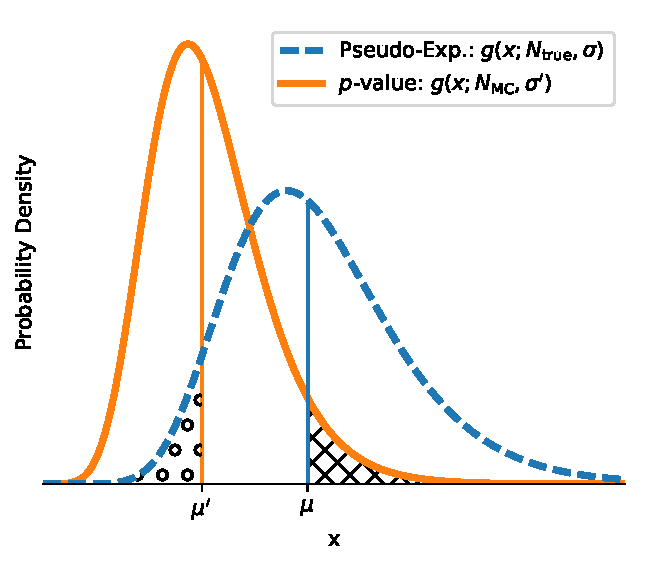
\includegraphics[width=0.7\textwidth]{coverage/coverage_distributions}
    \caption{Difference in widths of distributions while keeping the probabilities constant.}
    \label{fig:coverage_distributions}
\end{figure}


We find that a distribution set up at the new pseudo mean $\mu'$ with the same error parameter $\sigma$ does (in general) \emph{not} contain $\mu$ with the same probability as the original distribution around $\mu$ contained $\mu'$.
In order to fix that, one has to adapt the width of the distribution, e.g. the error parameter, to yield the same confidence interval.

The adjustment $\sigma \rightarrow \sigma'$ will be derived in the following:
Starting with the assumption that the probability of obtaining $\mu'$ given $\mu$ should be the same as obtaining $\mu$ given $\mu'$, we will derive an expression for $\sigma'$ such that
\begin{equation}
    P(x \leq \mu'; \mu, \sigma) = P(x \geq \mu; \mu', \sigma')
\end{equation}
This requirement can also be motivated in \fref{fig:coverage_distributions}, where the left-hand-side of the equation corresponds to the area filled with circles and the right-hand-side corresponds to the cross-hatched area under the probability distribution curve.

Let $g(x; \mu, \sigma)$ be the original distribution and $G(x; \mu; \sigma)$ its cumulative distribution function. The left-hand-side now spells out:
\begin{equation}
    P(x \leq \mu'; \mu, \sigma) = \int_0^{\mu'} g(x; \mu, \sigma) \dd{x} = G(\mu'; \mu, \sigma) - G(0; \mu, \sigma)
\end{equation}
Consequently, the right-hand-side corresponds to:
\begin{equation}
    P(x \geq \mu; \mu', \sigma) = \int_\mu^\infty g(x; \mu', \sigma') \dd{x} = G(\infty; \mu', \sigma') - G(\mu; \mu', \sigma')
\end{equation}
Since $G$ is a cumulative distribution function, we can substitute $G(0) = 0$ and $G(\infty) = 1$ and set both sides equal:
\begin{equation}
    G(\mu'; \mu, \sigma) = 1 - G(\mu; \mu', \sigma')
\end{equation}

\subsubsection{General Ideas}


\begin{align}
    \Phi(x) &= \frac{1}{2} \left(1+\erf\left(\frac{x}{\sqrt{2}}\right)\right) \\
    \Phi^{-1}(x) &= \sqrt{2}\,\erf^{-1}(2x - 1) 
\end{align}

\begin{align}
    \erf(x) &= \frac{2}{\sqrt{\pi}} \int_0^x e^{-t^2} \dd{t} \\
    \erf(-x) &= -\erf(x)
\end{align}


\begin{align}
    \Phi(x) &= 1 - \Phi(x') \\
    \Rightarrow x' &= \Phi^{-1}(1 - \Phi(x)) \\
    &= \sqrt{2} \erf^{-1}\left(2 \cdot \left[1 - \frac{1}{2} \left(1+\erf\left(\frac{x}{\sqrt{2}}\right)\right)\right]-1\right) \\
    %&= \sqrt{2}\erf^{-1}\left(2-1-\erf\left(\frac{x}{\sqrt{2}}\right)-1\right) \\
    &= \sqrt{2}\erf^{-1}\left(-\erf\left(\frac{x}{\sqrt{2}}\right)\right) \\
    &= \sqrt{2}\erf^{-1}\left(\erf\left(\frac{-x}{\sqrt{2}}\right)\right) \\
    &= -x
\end{align}


\subsubsection{Normal Distribution}

\begin{equation}
    G(\mu'; \mu, \sigma) = \Phi\left(\frac{\mu' - \mu}{\sigma}\right); \quad
    G(\mu; \mu', \sigma') = \Phi\left(\frac{\mu - \mu'}{\sigma'}\right)
\end{equation}

\begin{align}
    \Phi\left(\frac{\mu' - \mu}{\sigma}\right) &= 1 - \Phi\left(\frac{\mu - \mu'}{\sigma'}\right) \\
    \Rightarrow \frac{\mu' - \mu}{\sigma} &= - \frac{\mu - \mu'}{\sigma'} \\
    \Rightarrow \sigma' &= \sigma
\end{align} 

\subsubsection{Log-Normal Distribution}

The argumentation for the log-normal distribution is similar. The cumulative distribution of the log-normal distribution is 
\begin{equation}
    G(x; \mu, \sigma) = \Phi\left(\frac{\ln x - \mu}{\sigma}\right)
\end{equation}
Following the same argumentation, one obtains that again $\sigma$ must be conserved. However, in contrast to the case of the normal distribution, $\sigma$ now only depends on the \emph{relative} uncertainty (see \fref{eq:log_normal_substitution}).

Overall, one can conclude that the requirements on the distributions are met if the absolute error (in case of the normal distribution) or the relative error (in case of the log-normal distribution) are conserved.
